\documentclass[a4paper,12pt]{article} 


\usepackage[T2A]{fontenc}			% кодировка
\usepackage[utf8]{inputenc}			% кодировка исходного текста
\usepackage[english,russian]{babel}	% локализация и переносы


% Математика
\usepackage{amsmath,amsfonts,amssymb,amsthm,mathtools} 

\usepackage{gensymb}	
\usepackage{wasysym}

% Картинки
\usepackage{graphicx}
\graphicspath{{images/}}

%Заговолок
\usepackage[left=2cm,right=2cm,
    top=2cm,bottom=2cm,bindingoffset=0cm]{geometry}

\usepackage{titling}


\author{Петров Артём Антонович, группа 721}
\title{Лабораторная работа № 3.4.5 "Петля гистерезиса (динамический метод)"}
\date{\today}

%%%
\setlength{\parindent}{0pt}
%%%

\begin{document} % начало документа

\begin{minipage}[t][7cm]{\textwidth}
\maketitle
\end{minipage}

%
%\textbf{Цель работы:} 
%\bigskip
%
%\medskip
%\textbf{Оборудование:} 
%\bigskip
%
%\subsection*{Теоретическое введение}
%\bigskip
%

\bigskip

\subsection*{Экспериментальная установка}

\bigskip

\begin{figure}[ht]
\centering
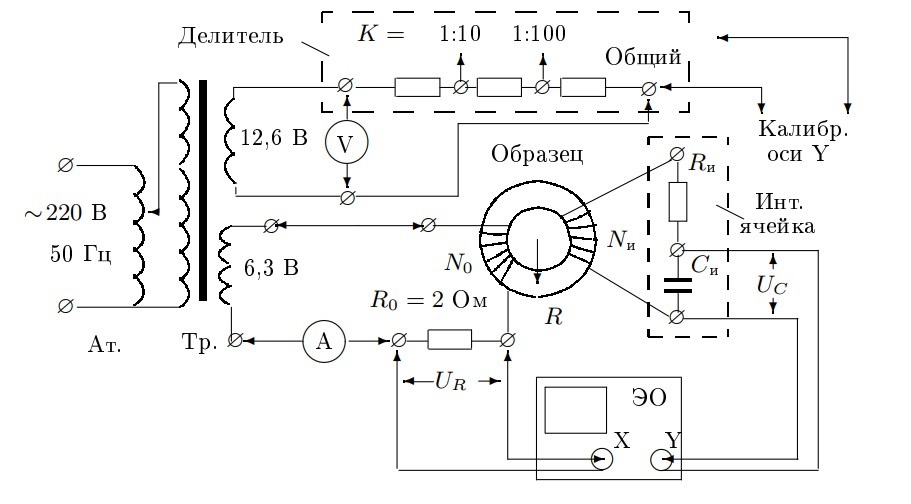
\includegraphics[width=140mm]{scheme.png}
\caption{Схема установки для изучения петли гистерезиса и калебровки приборов}\label{schema}
\end{figure}

В этой работе величины $K_x$ и $K_y$ указаны на Большое деление, в то время как все деления указаны в величинах маленьких делений, которые в 5 раз меньше больших.

Параметры установки:

$R_0 = 0.220 \pm 0.002 Ohm$
$R_u = 20kOhm$
$C_u = 20 \mu F$
\medskip

Феррит 1000

$N_0 = 42$ витка
$N_U = 400 $ витков
$S = 3,0 cm^2$
$2\pi R = 25 cm$
\medskip

Пермаллой

$N_0 = 20$ витка
$N_U = 300 $ витков
$S = 0,76 cm^2$
$2\pi R = 13,3 cm$
\medskip

Кремнистое железо

$N_0 = 25$ витка
$N_U = 250 $ витков
$S = 2,0 cm^2$
$2\pi R = 11 cm$




\bigskip

\subsection*{Ход работы}
\bigskip

\subsubsection*{Исследование гистерезиса}

Феррит
\begin{figure}[ht]
\centering
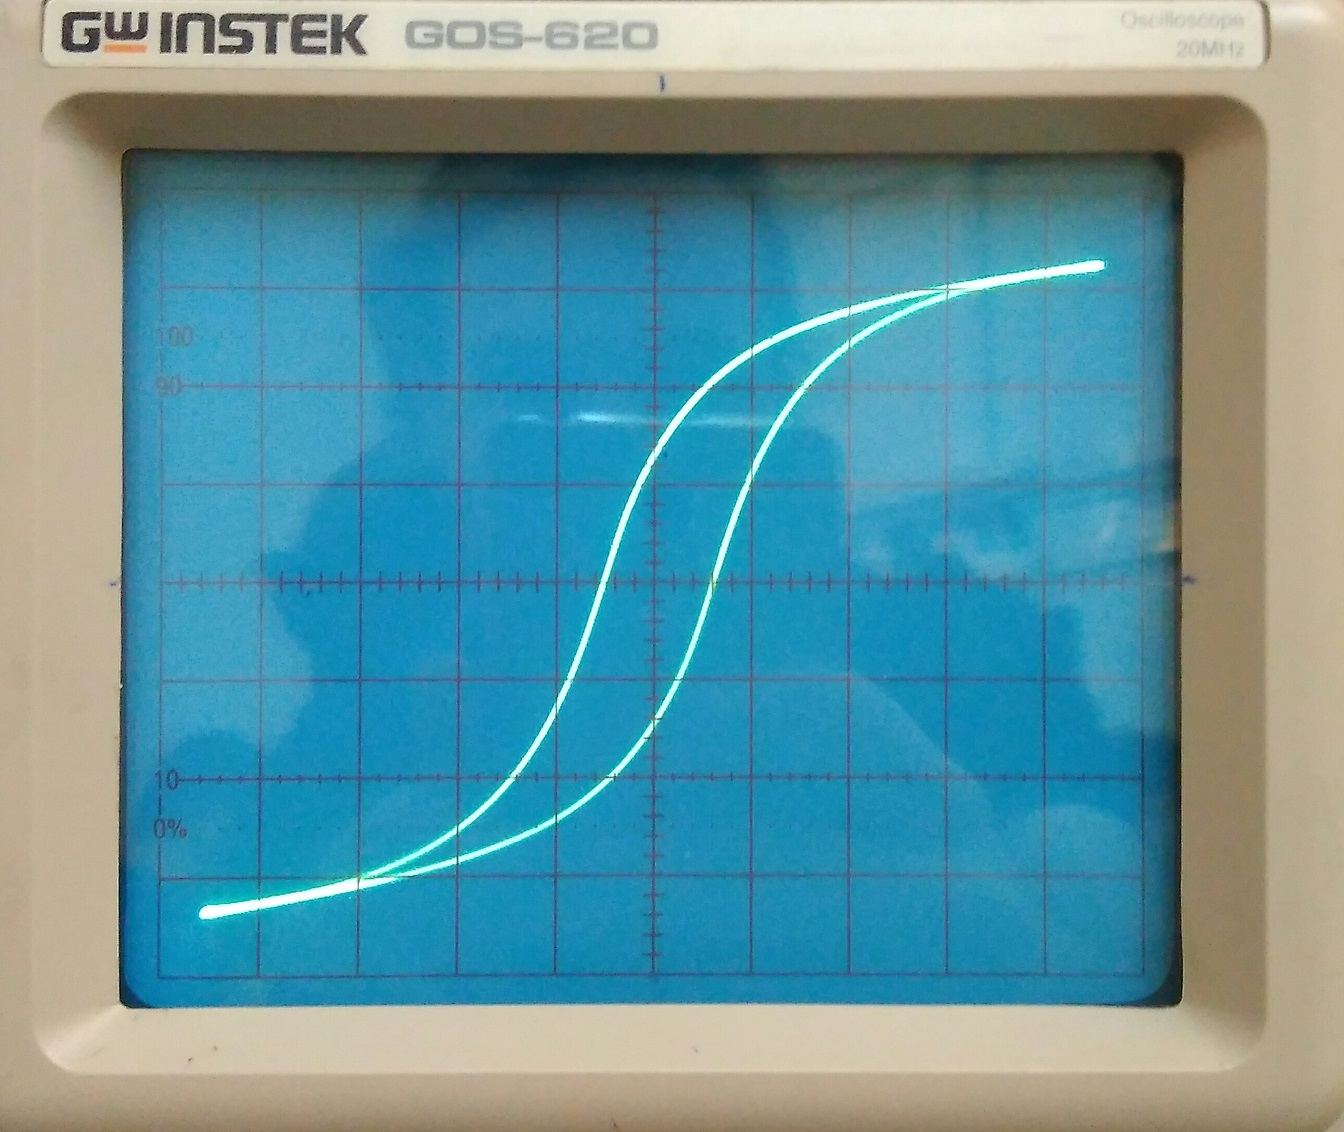
\includegraphics[width=100mm]{Ferrit.jpg}
\caption{Петля гистерезиса для образца из феррита}\label{schema}
\end{figure}

2)
$K_x = 50mV$
$K_y = 20mV$
$I_{eff} = 0.6454 \pm 0.0002 A$

3)Кривая снята при тех же $K_x; K_y$

4)
$2y = 36 del$
($K_y = 20mV$)
$2x = 30.5 del$
($K_x = 10 mV$)
\medskip

Пермаллой:

2)
$K_x = 20mV$
$K_y = 50mV$
$I_{eff} = 0.173 \pm 0.001 A$

3)Кривая снята при тех же $K_x; K_y$

4)
$2y = 17 del$
($K_y = 50mV$)
$2x = 36,5 del$
($K_x = 10 mV$)
\medskip

Кремнистое железо:

2)
$K_x = 0.1V$
$K_y = 50mV$
$I_{eff} = 1.252 \pm 0.002 A$

3)Кривая снята при тех же $K_x; K_y$

4)
$2y = 22 del$
($K_y = 50mV$)
$2x = 32 del$
($K_x = 20 mV$)


\subsubsection*{Калибровка}

Ось Х:

$K_x = 50mV$
$2x = 50 del$
$I_{Eff} = 0,767 \pm 0,001$

Ось У:

$K_y  =20 mV$
$2y = 41 del$
$U_{eff} = 58,3 \pm 0,2 mV$

$K_y  = 50 mV$
$2y = 38 del$
$U_{eff} = 135,0 \pm 1 mV$

\subsubsection*{Определение $\tau$}



Вход:

$K_y = 1V$
$2y_\text{вх} = 38 del$

Выход:

$K_y = 10mV$
$2y_\text{вых} = 30 del$

\bigskip

\textbf{Записи из журнала:}
\bigskip


\bigskip

\subsection*{Итог}
\bigskip
 
\end{document} % конец документа